\documentclass{ximera}
\newcommand{\RR}{\mathbb R}
\renewcommand{\d}{\,d}
\newcommand{\dd}[2][]{\frac{d #1}{d #2}}
\renewcommand{\l}{\ell}
\newcommand{\ddx}{\frac{d}{dx}}
\newcommand{\dfn}{\textbf}
\newcommand{\eval}[1]{\bigg[ #1 \bigg]}

\author{Jim Talamo and Bart Snapp}

\outcome{Introduce the method of "Slice, Approximate, Integrate" to set up Riemann integrals}
\outcome{Find the bounded area between two curves.}
\outcome{Express the area between curves as an integral or sum of integrals with respect to $x$ or $y$.}
\outcome{Decide whether to integrate with respect to $x$ or $y$.}


\title[Dig-In:]{Area between curves}
 
\begin{document}
\begin{abstract}
  We compute the area of a region between two curves using the
  definite integral.
\end{abstract}
\maketitle


\vspace{3mm}

In this section, we deal only with continuous functions defined on closed, bounded integrals.  When working with this type of function, there is a natural notion of ``area" between

We introduce

%%%%FINISH THIS

\section{The Fundamental Theorem of Calculus and Areas}

We begin the section with a motivating reminder:

\textbf{Motivating Reminder:} The area between a continuous function $y=f(x)$ and the $x$-axis between $x=a$ and $x=b$ for the function shown below:

\begin{figure}[h!]
  \centering 
  \includegraphics[width=.30 \textwidth]{B.eps}
\end{figure}

\vspace{3mm}
When this question arises at this stage in calculus, we may use the Fundamental Theorem of Calculus to write this area as a definite integral: $$\displaystyle A = \int_{x=a}^{x=b} f(x) \, dx .$$

However, recalling how this result was obtained in the first place is instructive and understanding the logic behind it is essential in order to apply a similar method to set up integrals to model other types of situations.  We thus give a detailed conceptual outline of the argument here:

\vspace{3mm}
\textbf{Step 1: Slice}

Since we have expressed $y$ as an function of $x$, we slice with respect to the independent variable (input), that is we divide the area up into $n$ pieces of uniform width $\Delta x$\footnote{The uniformity is not required in general, but this is a topic beyond the scope of our course.  This assumption is chosen here to make the example more conceptually tractable.}.

\begin{figure}[h!]
  \centering 
  \includegraphics[width=.30 \textwidth]{BSlice.eps}
  \caption{We slice the area into $n$ piece, each of width $\Delta x$.}
\end{figure}


\textbf{Step 2: Approximate}

We cannot determine the exact area of the slice, but we can approximate that each slice is a rectangle whose heights are determined by the value of the function $y = f(x)$ at some $x$-value on the base of the rectangle. 
\begin{figure}[h!]
  \centering 
  \includegraphics[width=.30 \textwidth]{BApprox.eps}
   \caption{We approximate each slice as a rectangle.}
\end{figure}

\vspace{3mm}
The area $\Delta A_k$ of one the $k$th rectangles is given by: 
\begin{align}
\Delta A_k & = (height) \times (width) \nonumber \\
\Delta A_k &= f\left(x_k^*\right)\Delta x \label{area}
\end{align}
where $x_k^*$ is the $x$-value in the chosen rectangle that determines its height $f(x_k^*)$. 

\vspace{3mm}
Let $S_n$ denote the total area obtained by adding the areas of the $n$ rectangles together.   Then, we can compute $S_n$ easily by adding up the areas of all of the rectangles: $$S_n = \Delta A_1 + \Delta A_2 + \ldots \Delta A_n$$
or if you prefer using sigma notation: 
\begin{equation}
S_n =\sum_{k=1}^{n} \Delta A_k =  \sum_{k=1}^n f(x_k^*) \Delta x  \label{areasum}
\end{equation}
Note that as we use more rectangles, the following occur \emph{simultaneously}:

\begin{itemize}
\item[1.] The width $\Delta x$ of each rectangle decreases.
\item[2.] The total number of rectangles increases.
\item[3.] The sum of the areas of the rectangles becomes closer to the actual area.
\end{itemize}

The actual area $A$ is indeed what we expect it should be: $$A = \lim_{n \rightarrow \infty} \left[ \sum_{k=1}^n f(x_k^*) \Delta x \right].$$ 

\vspace{3mm}
\textbf{Step 3: Integrate}

While this can be quite cumbersome to work out in even the simplest cases, the Fundamental Theorem of Calculus comes to the rescue; it guarantees that since $y=f(x)$ is continuous on $[a,b]$, this area is also computed via: $$A = \int_{x=a}^{x=b} f(x) \, dx$$
This can now be interpreted as follows:
\begin{itemize}
\item[1.] The integrand $f(x) \, dx$ is the area of an \emph{infinitesimal} rectangle of height $f(x)$ and thickness $dx$.\footnote{The notation ``$\Delta x$" represents the \emph{finite} but small width of a rectangle.  The notation ``$dx$" represents the \emph{infinitesimal} width of a rectangle and cannot be thought of strictly as 0!  This results from the area procedure the number of rectangles whose areas we must add increases \emph{simultaneously} without bound as the widths of each rectangle becomes arbitrarily close to 0!}
\item[2.] The procedure of definite integration can be thought of conceptually as \emph{simultaneously} shrinking the widths of the rectangles while adding them all together!
\end{itemize}
A similar procedure can be taken in many other examples for the rest of the chapter! The major point here is that once we find the approximate area for a \emph{single} rectangle in Eqn (\ref{area}), we can immediately write down the integral that gives the \emph{exact} area of the region by converting the $\Delta x$ in Eqn (\ref{areasum}) and the sum into a definite integral whose lower limit is the leftmost $x$-value in the region and whose righthand limit is the rightmost $x$-value in the region!


%%%%%%%%%%%%%%%%%%%%%%%%%%%%%%


\section{The Area Between Two Curves}

We have seen how integration can be used to find signed area between a curve and the $x$-axis. The above procedure can be used to find areas between curves.  Generally, we should interpret ``area'' as a positive quantity; all of the area bounded by the curves should be taken to be positive regardless of which the quadrant it appears!

Suppose now that we have two functions, $y=4x^3+17$ and $y=3x^2$ and suppose we want to find the area between the two curves on $[-1,1]$.  The area is shown below:

%%%%%%%ADD HANS PICTURE%%%%%%%%%%%%%





So should we do this? Let's apply the procedure of ``Slice, Approximate, Integrate".

\textbf{Step 1: Slice}

We divide the area up into $n$ pieces of uniform width $\Delta x$.

%%%%%%%HANS PICTURE%%%%%%%%%%%%%

\textbf{Step 2: Approximate}

We cannot determine the exact area of the slice, but just as before, we can approximate that each slice is a rectangle whose heights are determined by the value of the function $y = f(x)$ at some $x$-value on the base of the rectangle: 

%%%%%%%HANS PICTURE%%%%%%%%%%%%%

\vspace{3mm}
The area $\Delta A_k$ of one the $k$th rectangles is given by: 
\begin{align*}
\Delta A_k & = (height) \times (width) \nonumber \\
\end{align*}
where $x_k^*$ is the $x$-value in the chosen rectangle that determines its height $f(x_k^*)$. 

The height of the darkly shaded rectangle can be found by realizing that it is the change of $y$-values on the individual curves. In fact, if we consider a specific $x$-value in $[-1,1]$:

\begin{question}
The function used to determine the top $y$-value, $y_{top}$ is:
\begin{multipleChoice}
\choice[correct]{$y_{top}=4x^3+17$}
\choice{$y_{bot}=3x^2$}
\end{multipleChoice}
\end{question}

\begin{question}
The function used to determine the bottom $y$-value, $y_{bot}$ is:
\begin{multipleChoice}
\choice{$y_{top}=4x^3+17$}
\choice[correct]{$y_{bot}=3x^2$}
\end{multipleChoice}
\end{question}

Thus, the height $h$ of the rectangle is thus $h=y_{top}-y_{bot} = \answer[given]{(4x^3+17)-(3x^2)}$.

The approximate total area obtained by adding the areas of the $n$ rectangles between $x=-1$ and $x=1$ together.  Note that as we use more rectangles, the following occur \emph{simultaneously}:

\begin{itemize}
\item[1.] The width $\Delta x$ of each rectangle decreases.
\item[2.] The total number of rectangles increases.
\item[3.] The sum of the areas of the rectangles becomes closer to the actual area.
\end{itemize}

The actual area $A$ is indeed what we expect it should be: $$A = \lim_{n \rightarrow \infty} \left[ \sum_{k=1}^n f(x_k^*) \Delta x \right].$$ 

\vspace{3mm}
\textbf{Step 3: Integrate}

The same logic behind the Fundamental Theorem of Calculus allows us to write the above limit as a definite integral!  In fact:

\[
A = \int_{x=-1}^{x=1} (4x^3+17)-(3x^2) \d x
\]
By evaluating this, we can find the actual area:

\begin{align*}
A &= \int_{x=-1}^{x=1} 4x^3-3x^2+17 \d x \\
&= \eval{ x^4-x^3+17x}_{x= -1}^{x=1} \\
&= \left[(1)^4-(1)^3+17(1)\right] -  \left[(-1)^4-(-1)^3+17(-1)\right] \\
&=32
\end{align*}


Note that $A = \int_{x=-1}^{x=1} (4x^3+17)-(3x^2) \d x$ can be interpreted as follows:
\begin{itemize}
\item[1.] The integrand is the area of an \emph{infinitesimal} rectangle, whose height is determined as the difference between the top and bottom $y$-values of the bounding curves, and whose thickness $dx$. 
\item[2.] Since we integrate with respect to $x$, the limits of integration tell us the range of $x$-values the rectangles to be added are:
\begin{itemize}
\item The lower limit gives the $x$-value of the first slice.
\item The upper limit gives the $x$-value of the last slice.
\end{itemize}
\end{itemize}
We explicitly write $\int_{x=-1}^{x=1} (\ldots) \d x $ instead of $\int_{-1}^1(\ldots) \d x $ to make the fact that these limits correspond to $x$. 


\textbf{Remark:} Since the thickness is $\d x$, we MUST express the curves as functions of $x$; that is, we MUST write $y_{top}$ and $y_{bot}$ in terms of $x$!
 
A common theme that runs throughout this chapter is that once we choose a variable of integration, EVERY quantity (limits of integration, functions in the integrand) MUST be written in terms of that variable!


A similar procedure can be taken in many other examples for the rest of the chapter! The major point here is that once we find the approximate area for a \emph{single} rectangle, we can immediately write down the integral that gives the \emph{exact} area of the region!













%%%%%%%%%%%%%%%%%%COMMENT OUT%%%%%%%%%%%%%%%%%%%%%%%%

\begin{comment}
From the graph above we see that the area we want is the area under
$f$ minus the area under $g$, which is to say
\begin{align*}
\mathrm{Area} &= \int_a^b f(x)\d x-\int_a^b g(x)\d x \\
&= \int_a^b f(x)-g(x) \d x.
\end{align*}
It will also be useful to adopt the following intuitive way of
thinking about this problem: In a somewhat nonrigorous way, we can
think of an integral as ``summing up" an infinite number of
infinitesimal quantities. In this case we are summing rectangles of
width $\d x$ and height $f(x)-g(x)$:
\begin{image}
\begin{tikzpicture}
	\begin{axis}[
            domain=.5:2.5, ymax=10,xmax=2.5,ymin=0, xmin=.5,
            axis lines =left, xlabel=$x$, ylabel=$y$,
            xtick={1,2}, yticklabels={},
            ytick style={draw=none},
            xticklabels={$a$, $b$},
            width=4in,
            height=2in,
            every axis y label/.style={at=(current axis.above origin),anchor=south},
            every axis x label/.style={at=(current axis.right of origin),anchor=west},
            axis on top,
          ]
          %\addplot [draw=none,fill=fillp,domain=1:2] {-x^2+4*x+3} \closedcycle;
          %\addplot [draw=none,fill=background,domain=1:2] {-x^3 + 7*x^2-10*x+5} \closedcycle;
          \addplot [draw=penColor,very thick] {-x^2+4*x+3};
          \addplot [draw=penColor2,very thick] {-x^3 + 7*x^2-10*x+5};
          \node at (axis cs:1,6.7) [penColor] {$f$};
          \node at (axis cs:2,4) [penColor2] {$g$};
          \addplot [draw=penColor, fill = fillp] plot coordinates {(1.5,2.375) (1.6,2.375) (1.6, 6.84) (1.5,6.84) (1.5, 2.375)};
          
          \draw[decoration={brace,mirror,raise=.2cm},decorate,thin] (axis cs:1.5,2.7)--(axis cs:1.6,2.7);
          \node at (axis cs:1.55,1.25) {$\Delta x$};

          \draw[decoration={brace,raise=.2cm},decorate,thin] (axis cs:1.51,2.375)--(axis cs:1.51,6.84);
          \node[anchor=east] at (axis cs:1.45,4.6) {$f(x)-g(x)$};
        \end{axis}
\end{tikzpicture}
\end{image}
In this case, the integral
\begin{image}
  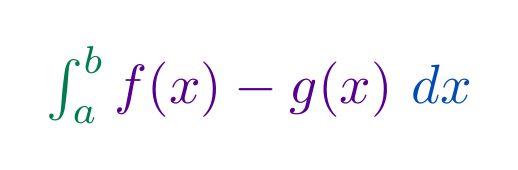
\begin{tikzpicture}[scale=2,every node/.style={transform shape}]
    \node at (0,0) {
      $\color{green!70!black!70!blue}\int_{a}^{b}\color{purple!50!blue!90!black}{f(x) - g(x)} \,\color{blue!70!green}{\d x}$
    };
  \end{tikzpicture}
\end{image}
could be interpreted as:
\begin{quote}
  \large\textbf{The \textcolor{green!70!black!70!blue}{sum} of the
    area of rectangles whose
    \textcolor{purple!50!blue!90!black}{heights are the difference
      between the top curve and bottom curve}, and whose
    \textcolor{blue!70!green}{widths are infinitesimal}.}
\end{quote}
This way of thinking about integrals will be very useful to us in
later, more complex, applications.

\end{comment}

%%%%%%%%%%%%%%%%%%%%%%%%%%%%%%%%%%%%%

\section{Integrating with respect to \textit{x}}

We can summarize the above procedure neatly with a simple formula that respects the geometrical reasoning used to generate the area of a region:

\begin{theorem}
The area of a region bounded by continuous functions is given by: 

\[A=\int_{x=a}^{x=b} h \d x \]

\end{theorem}

Let's look at a few more examples:


%%%%%%%%%MAke the below the exercise, make the exercise the actual example%%%%%%%%%%%%%%%%%%

\begin{example}
  Compute the area between $y=-x^2+4x+3$ and $=-x^3+7x^2-10x+5$ them on the interval $1 \le x \le 2$.
  
  We start by drawing the region in question, then indicate that we will build the area using vertical slices: 
    
\begin{image}
\begin{tikzpicture}
	\begin{axis}[
            domain=.5:2.5, ymax=10,xmax=2.5,ymin=0, xmin=.5,
            axis lines =left, xlabel=$x$, ylabel=$y$,
            xtick={1,2},
            ytick style={draw=none},
            width=4in,
            height=2in,
            yticklabels={},
            xticklabels={$1$, $2$},
            every axis y label/.style={at=(current axis.above origin),anchor=south},
            every axis x label/.style={at=(current axis.right of origin),anchor=west},
            axis on top,
          ]
          \addplot [draw=none,fill=fillp,domain=1:2] {-x^2+4*x+3} \closedcycle;
          \addplot [draw=none,fill=background,domain=1:2] {-x^3 + 7*x^2-10*x+5} \closedcycle;
          \addplot [draw=penColor,very thick] {-x^2+4*x+3};
          \addplot [draw=penColor2,very thick] {-x^3 + 7*x^2-10*x+5};
          \node at (axis cs:1.4,7.7) [penColor] {$y= -x^2+4x+3$};
          \node at (axis cs:1.7,1) [penColor2] {$y=-x^3+7x^2-10x+5$};
          
          \addplot [draw=penColor, fill = gray!50] plot coordinates {(1.5,2.375) (1.6,2.375) (1.6, 6.84) (1.5,6.84) (1.5, 2.375)};
          
        

          \draw[decoration={brace,raise=.2cm},decorate,thin] (axis cs:1.51,2.375)--(axis cs:1.51,6.84);
          \node[anchor=east] at (axis cs:1.45,4.6) {$h$};
          
          
        \end{axis}
\end{tikzpicture}
\end{image}
\begin{explanation}
 Consider the rectangle shown at an $x$-value in the interval of integration. We need to find the height of the rectangle in terms of $x$.  Once again, we find this by subtracting the top and bottom $y$-values on the curves:
 
 \begin{question}
The function used to determine the top $y$-value, $y_{top}$ is:
\begin{multipleChoice}
\choice[correct]{$y_{top}=-x^2+4x+3$}
\choice{$y_{bot}=-x^3 + 7x^2-10x+5$}
\end{multipleChoice}
\end{question}

\begin{question}
The function used to determine the bottom $y$-value, $y_{bot}$ is:
\begin{multipleChoice}
\choice{$y_{top}=-x^2+4x+3$}
\choice[correct]{$y_{bot}=-x^3 + 7x^2-10x+5$}
\end{multipleChoice}
\end{question}

Thus, the height $h$ of the rectangle is thus $h=y_{top}-y_{bot} = \answer[given]{(-x^2+4x+3)-(-x^3 + 7x^2-10x+5)}$.
 
We can now find the area:

\begin{align*}
A = \int_{x= a}^{x=b} h \d x &= \int_{x= \answer[given]{1}}^{x= \answer[given]{2}} (-x^2+4x+3)-(-x^3 + 7x^2-10x+5) \d x \\
  &=\int_1^2 \answer[given]{x^3-8x^2+14x-2} \d x \\
  &=\eval{\frac{x^4}{4}-\frac{8x^3}{3}+7x^2-2x}_1^2 \\
  &= \frac{16}{4} - \frac{64}{3}+28-4-(\frac{1}{4}- \frac{8}{3}+7-2) \\
  &=23-\frac{56}{3}-\frac{1}{4}\\
  &=\frac{49}{12}
\end{align*} 
 

\end{explanation}
\end{example}

%%%%%%%%%%%%%%%%%%%%%%%%%%%%%%%%







%%%%%%THIS EXAMPLE IS NOT COMPUTATIONALLY TRACTABLE  SAVE FOR EXERCISES%%%%%%%%%
\begin{comment}

In our first example, one curve was higher than the other over the
entire interval. This does not always happen.

\begin{example} Find the area between $f(x)= -x^2+4x$ and
$g(x)=x^2-6x+5$ over the interval $0 \le x \le 1$.


\begin{image}
\begin{tikzpicture}
	\begin{axis}[
            domain=-1:2, ymax=6,xmax=1.5,ymin=-0.3, xmin=-.5,
            axis lines =center, xlabel=$x$, ylabel=$y$,
	   xtick={0.5635,1},
            xticklabels={$a$,$1$}, 
            every axis y label/.style={at=(current axis.above origin),anchor=south},
            every axis x label/.style={at=(current axis.right of origin),anchor=west},
            axis on top,
          ]
          \addplot [draw=none,fill=fillp,domain=0:0.56] {x^2-6*x+5} \closedcycle;
          \addplot [draw=none,fill=background,domain=0:0.56] {-x^2+4*x} \closedcycle;
          \addplot [draw=none,fill=fillp,domain=0.56:1] {-x^2+4*x} \closedcycle;
          \addplot [draw=none,fill=background,domain=0.56:1] {x^2-6*x+5} \closedcycle;
          \addplot [draw=penColor,very thick] {-x^2+4*x};
          \addplot [draw=penColor2,very thick] {x^2 - 6*x+5};
          \node at (axis cs:1.25,3.1) [penColor] {$f$};
          \node at (axis cs:.25,4.3) [penColor2] {$g$};
          \addplot [textColor,dashed] plot coordinates {(0.5635,0) (0.5635,1.9364)};

        \end{axis}
\end{tikzpicture}
\end{image}


\begin{explanation}
Since the two curves cross, we need to compute two areas and add
them. First we find the intersection point of the curves.  Letting $a$
be the $x$-coordinate of the point of intersection, we have $a =
\answer[given]{\frac{5-\sqrt{15}}{2}}$

\begin{hint}
\begin{align*}
  -a^2+4a &= a^2-6a+5 \\
  0 &= 2a^2-10a+5 \\
  a &= \frac{10 \pm \sqrt{100-40}}{4}\\
 a &= \frac{5 \pm \sqrt{15}}{2}.
\end{align*}

Of the two solutions, only $\frac{5-\sqrt{15}}{2}$ is within the region of interest.
\end{hint}
Then the total area is 
\[
\textrm{Area} = \int_0^a g(x) - f(x) \d x + \int_a^1 f(x) - g(x) \d x
\]
since $g$ is above $f$ on the interval $[0,a]$, and $f$ is above $g$
on the interval $[a,1]$.  Computing this area we find
\[
\textrm{Area} = \answer[given]{5\sqrt{15} - \frac{52}{3}}.
\]
\begin{hint}
  \[
  \int_0^a g(x) - f(x) \d x + \int_a^1 f(x) - g(x) \d x
  \]
  \begin{align*}
    = \int_0^a & \answer{x^2-6x+5}-(-x^2+4x)\d x \\
    &+\int_a^1 \answer{-x^2+4x}-(x^2-6x+5)\d x
  \end{align*}
  Simplifying we find
  \begin{align*}
    &=\int_0^a 2x^2-10x+5\d x+\int_a^1 -2x^2+10x-5\d x \\
    &= \eval{\frac{2x^3}{3}-5x^2+5x}_0^a + \eval{ \frac{-2x^3}{3}+5x^2-5x}_a^1 \\
    &= 5\sqrt{15}-\frac{52}{3}.
  \end{align*}
\end{hint}
\end{explanation}
\end{example}

In both of our examples above, we gave you the limits of integration
by bounding the $x$-values between $0$ and $1$. However, in some problems
you will have to do more work to determine these bounds.

\begin{example}
Find the area bounded between $f(x)= -x^2+4x$ and $g(x)=x^2-6x+5$.
\begin{image}
\begin{tikzpicture}
	\begin{axis}[
            domain=0:5, ymax=5,xmax=5,ymin=-5, xmin=0,
            axis lines =center, xlabel=$x$, ylabel=$y$,
 	   xtick={0.5635},
            xticklabels={$a$}, 
            every axis y label/.style={at=(current axis.above origin),anchor=south},
            every axis x label/.style={at=(current axis.right of origin),anchor=west},
            axis on top,
          ]
          \addplot [draw=none,fill=fillp,domain=.56:4] {-x^2+4*x} \closedcycle;
          \addplot [draw=none,fill=fillp,domain=.56:4.44] {x^2-6*x+5} \closedcycle;
          \addplot [draw=none,fill=background,domain=4:5] {-x^2+4*x} \closedcycle;
          \addplot [draw=none,fill=background,domain=0:1] {x^2-6*x+5} \closedcycle;
          %\addplot [draw=none,fill=fillp,domain=.56:4] {-x^2+4*x} \closedcycle;       
          \addplot [draw=penColor,very thick,smooth] {-x^2+4*x};
          \addplot [draw=penColor2,very thick,smooth] {x^2-6*x+5};
          
          \node at (axis cs:2,4.4) [penColor] {$f$};
          \node at (axis cs:1,-1) [penColor2] {$g$};
	 \node at (axis cs:4.43649,0.3) [textColor] {b};
	 \addplot [textColor,dashed] plot coordinates {(0.5635,0) (0.5635,1.9364)};
          \addplot [textColor,dashed] plot coordinates {(4.43649,0) (4.43649,-1.9364)};
        \end{axis}
\end{tikzpicture}
\end{image}

\begin{explanation}
Here we are not given a specific interval, so it must be the case that
there is a ``natural'' region involved. Since the curves are both
parabolas, the only reasonable interpretation is the region between
the two intersection points, which we found in the previous example to
be $a=\answer[given]{(5-\sqrt{15})/2}$ and
$b=\answer[given]{(5+\sqrt{15})/2}$.  Since $f \ge g$ on $[a,b]$, the
geometric area is
\[
\int_a^b f(x) - g(x) \d x = \answer[given]{5\sqrt{15}}.
\]
\begin{hint}
\begin{align*}
  \int_a^b -x^2+4x-(x^2-6x+5)\d x
  &=\int_a^b -2x^2+10x-5\d x \\
  &=\eval{\answer{\frac{-2x^3}{3}+5x^2-5x}}_a^b \\
  &=\answer{5\sqrt{15}}.
\end{align*}
\end{hint}
\end{explanation}
\end{example}
\end{comment}

%%%%%%%%%%END OF COMMENTED OUT STUFF%%%%%%%%%%%%%%%%%%

\begin{example} Set up, bu do not evaluate, an integral or sum of integrals that expresses the area bounded by $y=\sqrt{x}$, $y=10-2x$ and $y=0$.

As usual, we begin by drawing a picture and indicating the type of rectangle that will be used to build the area:

\begin{image}
\begin{tikzpicture}
	\begin{axis}[
            domain=0:5.5, ymax=2.5,xmax=5.5, ymin=0, xmin=0,
            axis lines =center, xlabel=$x$, ylabel=$y$,
            every axis y label/.style={at=(current axis.above origin),anchor=south},
            every axis x label/.style={at=(current axis.right of origin),anchor=west},
            axis on top,
          ]
          \addplot [ fill = fillp, smooth, samples=100, domain=(0:2)] ({x^2},{x}) \closedcycle;
          \addplot [draw=none,fill=background,domain=0:5.2] {10-2*x} \closedcycle;   
          \addplot [very thick, penColor2, smooth, samples=100, domain=(0:3)] ({x^2},{x});
          \addplot [draw=penColor,very thick,smooth] {10-2*x};
          
          \node at (axis cs:3.4,1.7) [penColor2] {$g$};
          \node at (axis cs:4,0.7) [penColor] {$f$};
        \end{axis}
\end{tikzpicture}
\end{image}

As you can see, something interesting happens here!  The curve used to determine the height of the top rectangle changes!  In order to express this area by integrating with respect to $x$, we have to split it into two pieces:

%%%%HANS PICTURE%%%%%%%%%%

The top curve will change at the $x$-value where the two curves intersect.  Write with me:

\begin{align*}
\sqrt{x} &= 10-2x \\
x &= (10-2x)^2 \\
x&= 100-40x+4x^2 \\
4x^2-41x+100 &=0 \\
(4x-25)(x-4) &= 0
\end{align*}
Hence, $x=4$ or $x=\frac{25}{4}$.  Note that by squaring both sides to eliminate the square root, we may have introduced an extraneous root.  By substituting $x=4$ into the equation $\sqrt{x} = 10-2x$, we obtain $2=2$, which is a true statement.  However, doing the same for $x= \frac{25}{4}$ gives $\frac{5}{2} = -\frac{5}{2}$, which is not true!  Thus, we use $x=answer[given]{4}$.  

For the second region, we find the rightmost $x$-value is $x=5$ (which is done by setting $10-2x=0$).

\begin{tabular}{ll}
For Region I: \hspace{30mm} &  For Region II:  \\
$0 \le x \le 4$ & $4 \le x \le  5$\\
$y_{top} = \sqrt{x}$ & $y_{top} = 10-2x$ \\
$y_{bot} = 0$ & $y_{bot} = 0$ \\
$A_I = \int_{x= \answer[given]{0}}^{x=\answer[given]{4}} \answer[given]{x^{\frac{1}{2}}} \,d x$ & $A_{II} = \int_{x= \answer[given]{4}}^{x=\answer[given]{5}}  \answer[given]{10-2x} \,d x$
\end{tabular}

 Thus, $A= \int_{x= \answer[given]{0}}^{x=\answer[given]{4}} \answer[given]{x^{\frac{1}{2}}} \,d x + \int_{x= \answer[given]{4}}^{x=\answer[given]{5}}\answer[given]{10-2x} \,d x$
\end{example}


%%% ADD EXAMPLE BELOW AS INTEGRAL WRT x %%%%%%%%%%
\section{Integrating with respect to \textit{y}}

Consider the region bounded by the function $f(x) = x-3$, $g(x) =
\sqrt{x-1}$ and the horizontal axis:
\begin{image}
\begin{tikzpicture}
	\begin{axis}[
            domain=0:5.5, ymax=2.5,xmax=5.5, ymin=0, xmin=0,
            axis lines =center, xlabel=$x$, ylabel=$y$,
            every axis y label/.style={at=(current axis.above origin),anchor=south},
            every axis x label/.style={at=(current axis.right of origin),anchor=west},
            axis on top,
          ]
          \addplot [ fill = fillp, smooth, samples=100, domain=(0:2)] ({1+x^2},{x}) \closedcycle;
          \addplot [draw=none,fill=background,domain=0:5.2] {x-3} \closedcycle;   
          \addplot [very thick, penColor2, smooth, samples=100, domain=(0:3)] ({1+x^2},{x});
          \addplot [draw=penColor,very thick,smooth] {x-3};
          
          \node at (axis cs:3.4,1.7) [penColor2] {$g$};
          \node at (axis cs:4,0.7) [penColor] {$f$};
        \end{axis}
\end{tikzpicture}
\end{image}

While we could find the area of this region by breaking the
computation up into the two regions $[1,3]$ and $[3,5]$ (check that
$5$ is the intersection point!), there is another approach.  We can
think of splitting the region up into \textbf{horizontal} rectangles.

We can rewrite $y = \sqrt{x-1}$ as $x = y^2+1$, and we can rewrite $y
= x-3$ as $x = y+3$, so we have the following picture:

\begin{image}
\begin{tikzpicture}
	\begin{axis}[
            domain=0:5.5, ymax=2.5,xmax=5.5, ymin=0, xmin=0,
            axis lines =center, xlabel=$x$, ylabel=$y$,
            every axis y label/.style={at=(current axis.above origin),anchor=south},
            every axis x label/.style={at=(current axis.right of origin),anchor=west},
            axis on top,
          ]
          %\addplot [ fill = fillp, smooth, samples=100, domain=(0:2)] ({1+x^2},{x}) \closedcycle;
          %\addplot [draw=none,fill=background,domain=0:5.2] {x-3} \closedcycle;   
          \addplot [very thick, penColor2, smooth, samples=100, domain=(0:3)] ({1+x^2},{x});
          \addplot [draw=penColor,very thick,smooth] {x-3};
          
          \node at (axis cs:3.4,1.7) [penColor2] {$g$};
          \node at (axis cs:4,0.7) [penColor] {$f$};

	  \addplot [draw=penColor, fill = fillp] plot coordinates {(2,1) (2,1.1) (4, 1.1) (4,1) (2, 1)};

          \draw[decoration={brace,raise=.2cm},decorate,thin] (axis cs:2,1)--(axis cs:2,1.1);
          \node at (axis cs:1.6,1.05) {$\d y$};

          \draw[decoration={brace,mirror,raise=.2cm},decorate,thin] (axis cs:2,1)--(axis cs:4,1);
          \node at (axis cs:2.7,.7) {$f^{-1}(y)-g^{-1}(y)$};
        \end{axis}
\end{tikzpicture}
\end{image}
In this case, the integral
\begin{image}
  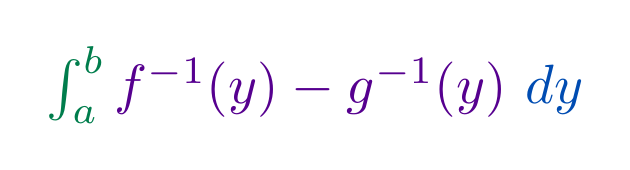
\begin{tikzpicture}[scale=2,every node/.style={transform shape}]
    \node at (0,0) {
      $\color{green!70!black!70!blue}\int_{a}^{b}\color{purple!50!blue!90!black}{f^{-1}(y) - g^{-1}(y)} \,\color{blue!70!green}{\d y}$
    };
  \end{tikzpicture}
\end{image}
could be interpreted as:
\begin{quote}
  \large\textbf{The \textcolor{green!70!black!70!blue}{sum} of the
    area of rectangles whose
    \textcolor{purple!50!blue!90!black}{widths are the difference
      between the right curve and left curve}, and whose
    \textcolor{blue!70!green}{heights are infinitesimal}.}
\end{quote}


Let's see an example.

\begin{example}
  Compute the area of the region bounded by the function $f(x) = x-3$,
  $g(x) = \sqrt{x-1}$ and the horizontal axis:
\begin{image}
\begin{tikzpicture}
	\begin{axis}[
            domain=0:5.5, ymax=2.5,xmax=5.5, ymin=0, xmin=0,
            axis lines =center, xlabel=$x$, ylabel=$y$,
            every axis y label/.style={at=(current axis.above origin),anchor=south},
            every axis x label/.style={at=(current axis.right of origin),anchor=west},
            axis on top,
          ]
          \addplot [ fill = fillp, smooth, samples=100, domain=(0:2)] ({1+x^2},{x}) \closedcycle;
          \addplot [draw=none,fill=background,domain=0:5.2] {x-3} \closedcycle;   
          \addplot [very thick, penColor2, smooth, samples=100, domain=(0:3)] ({1+x^2},{x});
          \addplot [draw=penColor,very thick,smooth] {x-3};
          
          \node at (axis cs:3.4,1.7) [penColor2] {$g$};
          \node at (axis cs:4,0.7) [penColor] {$f$};
        \end{axis}
\end{tikzpicture}
\end{image}
\begin{explanation}
  This area will be easier to compute if we look at $f^{-1}$ and $g^{-1}$. We have that
  \begin{align*}
    f^{-1}(y) &= \answer[given]{y+3}\\
    g^{-1}(y) &= \answer[given]{y^2 +1}
  \end{align*}
  We also must find where $f^{-1}$ and $g^{-1}$ intersect. Write with me
  \begin{align*}
    y+3 &= y^2 +1,\\
    \answer[given]{y^2-y-2} &= 0\\
    y &= -1 \text{ or }\answer[given]{2}.
  \end{align*}
  Note that $-1$ is not relevant for this problem.  Thus the area is
  given by
  \[
  \int_{0}^{2}(y+3) - (y^2+1)\d y = \answer[given]{\frac{10}{3}}.
  \]
  \begin{hint}
    \begin{align*}
      \int_0^2 (y+3) - (y^2+1) \d y &= \int_0^2 -y^2+y+2 \d y\\
      &=\eval{\answer{\frac{-y^3}{3} + \frac{y^2}{2}+2y}}_0^2\\
      &=\answer{\frac{10}{3}}.
    \end{align*}
  \end{hint}
\end{explanation}
\end{example}



%%%%%%%% ADD A FEW SET UP EXAMPLES %%%%%%%%%%%


\end{document}
